\begin{frame}{Projection onto a line}
\begin{itemize}
    \item \textbf{Vector projection onto a line}: Given a vector $x$, its projection $p$ onto a line spanned by vector $u$ is defined as 
    \begin{align}
        p = \frac{x^T u}{\|u\|^2}u
    \end{align}
    \item The residual $e = x - p$ is orthogonal to $u$, satisfying $u^Te = 0$.
    \item \textbf{Projection matrix}: The projection can be expressed as $p = Px$ where $P$ is the projection matrix:
    \begin{align}
        P = \frac{uu^T}{\|u\|^2} 
    \end{align}
 \end{itemize}
\end{frame}

\begin{frame}{}
\begin{center}
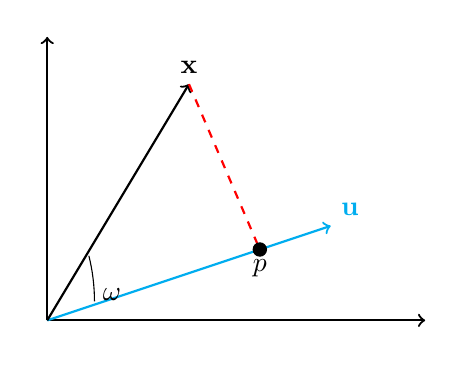
\begin{tikzpicture}[scale=1.2]
    % Axes
    \draw[->, thick] (0,0) -- (4,0) node[below] {};
    \draw[->, thick] (0,0) -- (0,3) node[left] {};
    
    % Direction vector u (cyan arrow)
    \draw[->, thick, cyan] (0,0) -- (3,1) node[above right] {$\mathbf{u}$};
    
    % Vector x (black arrow)
    \draw[->, thick] (0,0) -- (1.5,2.5) node[above] {$\mathbf{x}$};
    
    % Projection line (red dashed)
    \draw[dashed, red, thick] (1.5,2.5) -- (2.25,0.75);
    
    % Projection point
    \filldraw[black] (2.25,0.75) circle (2pt) node[below] {$p$};
    
    % Angle between u and x
    \draw (0.5,0.2) arc (0:14:2) node[midway, below right] {$\omega$};
\end{tikzpicture}
\end{center}
\begin{itemize}
\item \textbf{Example}: Consider vectors $x$ and $u$:
    \begin{align*}
        x = \begin{bmatrix}
            2\\3
        \end{bmatrix}, \quad u =\begin{bmatrix}
            1\\0
        \end{bmatrix}
    \end{align*}
    \item Since $\|u\|^2 = 1$ and $x^T u = 2 \cdot 1 + 3 \cdot 0 = 2$
\end{itemize}
\end{frame}

\begin{frame}{}
\begin{itemize}
    \item The projection is $p = 2\begin{bmatrix}
        1\\0
    \end{bmatrix} = \begin{bmatrix}
        2\\0
    \end{bmatrix}$
    \item \textbf{Matrix example}: For projection onto the line spanned by $b=[1, 2, 2]^T$:
    \begin{align}
        P = \frac{bb^T}{\|b\|^2} = \frac{1}{9} \begin{bmatrix}
            1\\ 2\\ 2 
        \end{bmatrix}\begin{bmatrix}
            1 & 2& 2 
        \end{bmatrix} = \frac{1}{9} \begin{bmatrix}
            1 & 2&2\\
            2&4 & 4\\
            2&4&4
        \end{bmatrix}
    \end{align}
    \item For any vector $x$, its projection onto this line is:
    \begin{align}
        p = Px = \frac{1}{9} \begin{bmatrix}
            1 & 2&2\\
            2&4 & 4\\
            2&4&4
        \end{bmatrix}\begin{bmatrix}
            x_1\\x_2 \\
            x_3
        \end{bmatrix} = \frac{1}{9} \begin{bmatrix}
            x_1 + 2x_2 + 2x_3\\
            2x_1 + 4x_2 + 4x_3\\
            2x_1 + 4x_2 + 4x_3
        \end{bmatrix}
    \end{align}
\end{itemize}
\end{frame}

\begin{frame}{Exercise}
\begin{enumerate}
    \item Calculate the projection vector $p$ and determine the projection matrix $P$ for the given vectors:
    \begin{align}
        a)\;\; x=\begin{bmatrix}
        1\\1\\1
    \end{bmatrix}, \;u=\begin{bmatrix}
        1\\2\\2
    \end{bmatrix}\;\; b) \;\;  x=\begin{bmatrix}
        1\\0\\1
    \end{bmatrix}, u=\begin{bmatrix}
        1\\-1\\2
    \end{bmatrix}
    \end{align}
    \item For both cases above, evaluate $P^2$ and $P^3$. What pattern do you notice?
    \item Verify that the residual $e=x-p$ is orthogonal to $u$, i.e., $u^Te=0$
    \item Demonstrate that $\|p\| = \|x\| \cos \theta$, where $\theta$ represents the angle between $x$ and $u$.
\end{enumerate}
\end{frame}


\begin{frame}{Projection onto a Plane}
\begin{itemize}
    \item \textbf{Projection of a vector onto a plane}: Given a vector $x$ and a 2D plane $\pi$, the projection of $x$ onto $\pi$ is a vector $x'$ given by
    \begin{align}
        x' = \frac{x^Tu}{\|u\|^2}u + \frac{x^Tv}{\|v\|^2}v
    \end{align}
    where $u$ and $v$ are orthogonal basis vectors spanning the plane.
    \item In matrix notation, the projection $x'$ of $x$ is:
    \begin{align}
        x' = \left( I - nn^T \right) x,
    \end{align}
    where $n$ is the unit normal vector to the plane, and $P = I - nn^T$ is the orthogonal projection matrix onto the plane.
\end{itemize}
\end{frame}

\begin{frame}{}
\begin{figure}
\begin{center}
    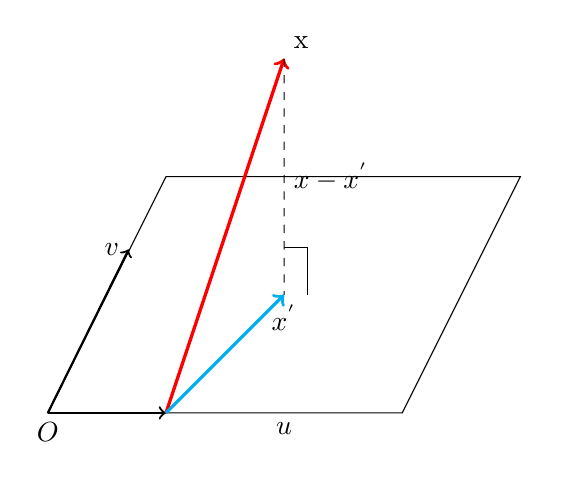
\begin{tikzpicture}[scale=1.5]
    % Define the parallelogram (plane) vertices
    \coordinate (A) at (0,0,0);
    \coordinate (B) at (3,0,0);  % Adjust for the slant of the parallelogram
    \coordinate (AB) at (1,0,0) node[below]{$O$};
    \coordinate (AD) at (0.3,1,-1);
    \coordinate (C) at (4,2,0);  % Adjust for the shape
    \coordinate (D) at (1,2,0);  
    \draw (2,0,0) node[below]{$u$};
    \draw (0.3,1,-1) node[left]{$v$};
    
    % Draw the parallelogram (plane)
    \draw (A) -- (B) -- (C) -- (D) -- cycle;
    \draw [->, thick](A) -- (AB);
    \draw[->, thick] (A)--(AD);
    
    % Label the corners of the parallelogram
    \node[below left] at (A) {};
    \node[below right] at (B) {};
    \node[above right] at (C) {};
    \node[above left] at (D) {};
    
    % Define the perpendicular line (normal to the plane) starting from the center of the parallelogram
    \coordinate (Center) at (2,1,0);  % Approximate center of the parallelogram
    \draw (2,3,0) node[above right]{x};
    \draw[->, very thick, red] (AB) --(2,3,0);
    \draw[->, very thick, cyan] (AB)-- (2,1,0);
    \draw[dashed] (2,3,0) -- (Center) node[midway, right]{$x-x^{'}$};
    \coordinate (Top) at (2,1.5,2);  
    \draw (2,1.4,0)--(2.2,1.4,0)--(2.2,1,0);
    \draw (2,1,0) node[below]{$x^{'}$};
    \end{tikzpicture}
    \caption{Projection onto a plane spanned by $u$ and $v$. The projection $x'$ can be expressed as a linear combination of $u$ and $v$.}
    \label{fig:enter-label}
\end{center}
\end{figure}
\end{frame}


\begin{frame}{}
    \begin{itemize}
        \item \textbf{Example}: Consider a plane with normal vector $n$ and a vector $x$ to be projected:
        \begin{align*}
            n = \begin{bmatrix}
                0\\0\\1
            \end{bmatrix}, \quad x = \begin{bmatrix}
                1\\2\\3
            \end{bmatrix}
        \end{align*}
        \item First, verify that $n$ is a unit vector: $\|n\| = 1$ (which is already the case).
        \item Calculate the outer product $nn^T$: 
        \begin{align*}
            nn^T = 
                \begin{bmatrix}
                0\\0\\1
            \end{bmatrix}\begin{bmatrix}0 & 0 & 1\end{bmatrix} = \begin{bmatrix}
                0 & 0 & 0\\
                0 & 0 & 0\\
                0 & 0 & 1
            \end{bmatrix}
        \end{align*}
        \item Determine the projection matrix $P$:
    \end{itemize}
\end{frame}




\begin{frame}{}
\begin{itemize}
    \item The projection matrix $P$ is: 
    \begin{align*}
        P = I - nn^T = \begin{bmatrix}
           1&0&0\\
           0&1&0\\
           0&0&1
        \end{bmatrix} - \begin{bmatrix}
             0 &0& 0\\
             0&0& 0\\
             0&0&1
          \end{bmatrix}= \begin{bmatrix}
             1 & 0 & 0\\
             0& 1& 0 \\
             0& 0& 0
          \end{bmatrix}
    \end{align*}
    \item The projection of $x$ onto the plane is:
    \begin{align*}
        x' = Px = \begin{bmatrix}
             1 & 0 & 0\\
             0& 1& 0 \\
             0& 0& 0
          \end{bmatrix}\begin{bmatrix}
             1\\2\\3
          \end{bmatrix} = \begin{bmatrix}
             1\\2\\0
          \end{bmatrix}
    \end{align*}
\end{itemize}
\end{frame}


\begin{frame}{Projection onto a Subspace}
    \begin{itemize}
        \item \textbf{General subspace projection}: Given $n$ linearly independent vectors $a_1, \ldots, a_n \in \mathbb{R}^m$, we seek the projection $p$ of vector $b$ onto the subspace spanned by these vectors:
        \begin{align}
            p = \hat{p}_1a_1 + \cdots + \hat{p}_na_n \label{proj1}
        \end{align}
        where the coefficients $\hat{p}_i$ are determined by the orthogonality condition.
        \item Let $A = [a_1 \; a_2 \; \cdots \; a_n]$ be the matrix with columns $a_i$. The projection coefficients satisfy:
        \begin{align}
            A^T(b-A\hat{p}) = 0 \quad \Rightarrow \quad A^TA\hat{p} = A^Tb
        \end{align}
        \item The projection onto the column space of $A$ is:
        \begin{align}
            p = A(A^TA)^{-1}A^Tb
        \end{align}
    \end{itemize}
\end{frame}

\begin{frame}{Projection onto General Subspaces}
    \begin{itemize}
        \item \textbf{Setting}: Let $x \in \mathbb{R}^n$ and $U \subset \mathbb{R}^n$ be a subspace with $\dim(U) = m \geq 1$.
        \item Let $\{b_1, b_2, \ldots, b_m\}$ be a basis for $U$, and define $B = [b_1 \; b_2 \; \cdots \; b_m]$.
        \item Any vector in $U$ can be written as:
        \begin{align*}
            x' = \sum_{i=1}^{m} \lambda_i b_i = B\lambda
        \end{align*}
        for some coefficient vector $\lambda = [\lambda_1, \ldots, \lambda_m]^T$.
    \end{itemize}
\end{frame}

\begin{frame}
    \begin{itemize}
        \item The orthogonal projection of $x$ onto $U$ is:
        \begin{align}
            x' = B(B^TB)^{-1}B^Tx
        \end{align}
        where $P = B(B^TB)^{-1}B^T$ is the projection matrix onto $U$.
    \end{itemize}
\end{frame}


\begin{frame}{Exercices}
\begin{enumerate}
    \item Given a vector $x = \begin{bmatrix} 1 \\ 2 \\ 3 \end{bmatrix}$ and a subspace spanned by $b_1 = \begin{bmatrix} 1 \\ 0 \\ 0 \end{bmatrix}$ and $b_2 = \begin{bmatrix} 0 \\ 1 \\ 0 \end{bmatrix}$, compute the projection of $x$ onto the subspace.
    \item For the same vectors, calculate the projection matrix $P$ and verify that $P^2 = P$.
    \item Show that the error vector $e = x - x'$ is orthogonal to both $b_1$ and $b_2$.
    \item Prove that the projection $x'$ satisfies $\|x'\| = \|b_1\| \cos \theta_1 + |b_2| \cos \theta_2$, where $\theta_1$ and $\theta_2$ are the angles between $x'$ and $b_1$, and $x'$ and $b_2$,
    respectively.
\end{enumerate} 
\end{frame}



